\documentclass[border=6pt]{standalone}
\usepackage{tikz}
\usetikzlibrary{arrows.meta,positioning,calc,shapes.geometric,fit,backgrounds,patterns,matrix,decorations.pathreplacing}
\begin{document}
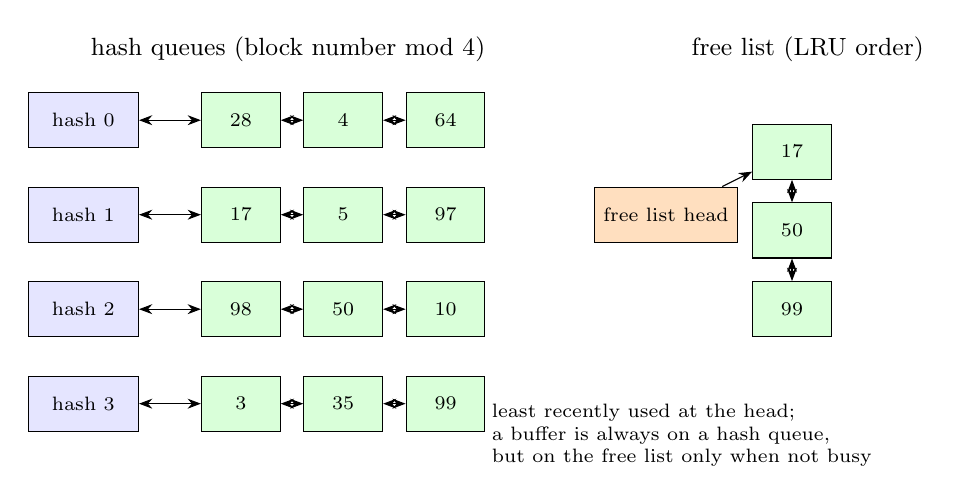
\begin{tikzpicture}[>=Stealth,font=\small]
\tikzstyle{h}=[draw,minimum width=1.4cm,minimum height=0.7cm,font=\scriptsize,fill=blue!10]
\tikzstyle{b}=[draw,minimum width=1.0cm,minimum height=0.7cm,font=\scriptsize,fill=green!15]
\node[font=\small] at (2.6,0.9) {hash queues (block number mod 4)};
\foreach \i/\x/\y/\z in {0/28/4/64,1/17/5/97,2/98/50/10,3/3/35/99} {
 \node[h] (h\i) at (0,-\i*1.2) {hash \i};
 \node[b] (a\i) at (2.0,-\i*1.2) {\x};
 \node[b] (b\i) at (3.3,-\i*1.2) {\y};
 \node[b] (c\i) at (4.6,-\i*1.2) {\z};
 \draw[<->] (h\i) -- (a\i); \draw[<->] (a\i) -- (b\i); \draw[<->] (b\i) -- (c\i);
}
\node[font=\small] at (9.2,0.9) {free list (LRU order)};
\node[h,fill=orange!25] (fh) at (7.4,-1.2) {free list head};
\node[b] (f1) at (9.0,-0.4) {17}; \node[b] (f2) at (9.0,-1.4) {50}; \node[b] (f3) at (9.0,-2.4) {99};
\draw[->] (fh) -- (f1); \draw[<->] (f1) -- (f2); \draw[<->] (f2) -- (f3);
\node[font=\scriptsize,align=left] at (7.6,-4.0) {least recently used at the head;\\ a buffer is always on a hash queue,\\ but on the free list only when not busy};
\end{tikzpicture}
\end{document}
